\documentclass[../main.tex]{subfiles}




\begin{document}

\chapter{}
\label{cha:cha_6}


\section{}


The function can be set up for fixed-point iteration by solving it for $x$
\bigbreak
$x_{i+1}=\sin \left(\sqrt{x_{i}}\right)$
\bigbreak
Using an initial guess of $x_{0}=0.5$, the first iteration yields
\bigbreak
$
\begin{aligned}
&x_{1}=\sin (\sqrt{0.5})=0.649637 \\\\
&\left|\varepsilon_{a}\right|=\left|\dfrac{0.649637-0.5}{0.649637}\right| \times 100 \%=23 \%
\end{aligned}
$
\bigbreak
Second iteration:
\bigbreak
$
\begin{aligned}
&x_{2}=\sin (\sqrt{0.649637})=0.721524 \\\\
&\left|\varepsilon_{a}\right|=\left|\dfrac{0.721524-0.649637}{0.721524}\right| \times 100 \%=9.96 \%
\end{aligned}
$
\bigbreak
The process can be continued as tabulated below:
\bigbreak
\begin{tabular}{crr}
\hline
iteration & \multicolumn{1}{c}{$x_{i}$} & \multicolumn{1}{c}{$\left|\varepsilon_{\mathrm{a}}\right|$} \\
\hline
0 & $0.500000$ &  \\
1 & $0.649637$ & $23.0339 \%$ \\
2 & $0.721524$ & $9.9632 \%$ \\
3 & $0.750901$ & $3.9123 \%$ \\
4 & $0.762097$ & $1.4691 \%$ \\
5 & $0.766248$ & $0.5418 \%$ \\
6 & $0.767772$ & $0.1984 \%$ \\
7 & $0.768329$ & $0.0725 \%$ \\
8 & $0.768532$ & $0.0265 \%$ \\
9 & $0.768606$ & $0.0097 \%$ \\
\hline
\end{tabular}
\bigbreak
Thus, after nine iterations, the root is estimated to be $0.768606$ with an approximate error of $0.0097 \%$.
\bigbreak


\section{}
\begin{enumerate}[label=\bfseries(\alph*)]
\item The function can be set up for fixed-point iteration by solving it for $x$ in two different ways. First, it can be solved for the linear $x$,



\bigbreak
$x_{i+1}=\dfrac{0.9 x_{i}^{2}-2.5}{1.7}$
\bigbreak
Using an initial guess of 5 , the first iteration yields
\bigbreak
$
\begin{aligned}
&x_{1}=\dfrac{0.9(5)^{2}-2.5}{1.7}=11.76 \\\\
&\left|\varepsilon_{a}\right|=\left|\dfrac{11.76-5}{11.76}\right| \times 100 \%=57.5 \%
\end{aligned}
$
\bigbreak
Second iteration:
\bigbreak
$
\begin{aligned}
&x_{1}=\dfrac{0.9(11.76)^{2}-2.5}{1.7}=71.8 \\\\
&\left|\varepsilon_{a}\right|=\left|\dfrac{71.8-11.76}{71.8}\right| \times 100 \%=83.6 \%
\end{aligned}
$
\bigbreak
Clearly, this solution is diverging.
\bigbreak
An alternative is to solve for the second-order $x$,
\bigbreak
$x_{i+1}=\sqrt{\dfrac{1.7 x_{i}+2.5}{0.9}}$
\bigbreak
Using an initial guess of 5 , the first iteration yields
\bigbreak
$
\begin{aligned}
&x_{i+1}=\sqrt{\dfrac{1.7(5)+2.5}{0.9}}=3.496 \\\\
&\left|\varepsilon_{a}\right|=\left|\dfrac{3.496-5}{3.496}\right| \times 100 \%=43.0 \%
\end{aligned}
$
\bigbreak
Second iteration:
\bigbreak
$
\begin{aligned}
&x_{i+1}=\sqrt{\dfrac{1.7(3.496)+2.5}{0.9}}=3.0629 \\\\
&\left|\varepsilon_{a}\right|=\left|\dfrac{3.0629-3.496}{3.0629}\right| \times 100 \%=14.14 \%
\end{aligned}
$
\bigbreak
This version is converging. All the iterations can be tabulated as
\bigbreak
$\begin{array}{ccc}\text { iteration } & x_{i} & \left|\varepsilon_{a}\right| \\ 0 & 5.000000 & \\ 1 & 3.496029 & 43.0194 \% \\ 2 & 3.062905 & 14.1410 \% \\ 3 & 2.926306 & 4.6680 \% \\ 4 & 2.881882 & 1.5415 \% \\ 5 & 2.867287 & 0.5090 \%\\ 6 & 2.862475 & 0.1681 \% \\ 7 & 2.860887 & 0.0555 \% \\ 8 & 2.860363 & 0.0183 \% \\ 9 & 2.860190 & 0.0061 \%\end{array}$
\bigbreak
Thus, after 9 iterations, the root estimate is $2.860190$ with an approximate error of $0.0061 \%$. The result can be checked by substituting it back into the original function,
\bigbreak
$f(2.860190)=-0.9(2.860190)^{2}+1.7(2.860190)+2.5=-0.000294$
\bigbreak
\item The formula for Newton-Raphson is
\bigbreak
$x_{i+1}=x_{i}-\dfrac{-0.9 x_{i}^{2}+1.7 x_{i}+2.5}{-1.8 x_{i}+1.7}$
\bigbreak
Using an initial guess of 5 , the first iteration yields
\bigbreak
$x_{i+1}=5-\dfrac{-0.9(5)^{2}+1.7(5)+2.5}{-1.8(5)+1.7}=3.424658$
\bigbreak
$\left|\varepsilon_{a}\right|=\left|\dfrac{3.424658-5}{3.424658}\right| \times 100 \%=46.0 \%$
\bigbreak
Second iteration:
\bigbreak
$x_{i+1}=3.424658-\dfrac{-0.9(3.424658)^{2}+1.7(3.424658)+2.5}{-1.8(3.424658)+1.7}=2.924357$
\bigbreak
$\left|\varepsilon_{a}\right|=\left|\dfrac{2.924357-3.424658}{2.924357}\right| \times 100 \%=17.1 \%$
\bigbreak
The process can be continued as tabulated below:
\bigbreak
\begin{tabular}{crrrc}
iteration & \multicolumn{1}{c}{$x_{i}$} & $f\left(x_{i}\right)$ & $f\left(x_{i}\right)$ & $\left|\varepsilon_{\mathrm{a}}\right|$ \\
0 & 5 & $-11.5$ & $-7.3$ &  \\
1 & $3.424658$ & $-2.23353$ & $-4.46438$ & $46.0000 \%$ \\
2 & $2.924357$ & $-0.22527$ & $-3.56384$ & $17.1081 \%$ \\
3 & $2.861147$ & $-0.00360$ & $-3.45006$ & $2.2093 \%$ \\
4 & $2.860105$ & $-9.8 \mathrm{E}-07$ & $-3.44819$ & $0.0364 \%$ \\
5 & $2.860104$ & $-7.2 \mathrm{E}-14$ & $-3.44819$ & $0.0000 \%$ \\
\end{tabular}
\bigbreak
After 5 iterations, the root estimate is $\mathbf{2 . 8 6 0 1 0 4}$ with an approximate error of $0.0000 \%$. The result can be checked by substituting it back into the original function,
\bigbreak
$f(2.860104)=-0.9(2.860104)^{2}+1.7(2.860104)+2.5=-7.2 \times 10^{-14}$
\bigbreak


\end{enumerate}


\section{}
\begin{enumerate}[label=\bfseries(\alph*)]
\item
\begin{lstlisting}[numbers=none]
>> x = linspace(0,4);
>> y = x.^3-6*x.^2+11*x-6.1;
>> plot(x,y)
>> grid
\end{lstlisting}
\bigbreak
	\begin{figure}[H]
		\hspace*{1.25cm}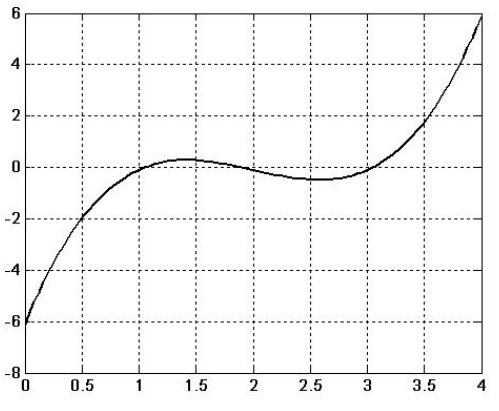
\includegraphics[width=0.5\linewidth]{fig_6_1}
		\label{fig:fig_6_1}
	\end{figure}
	\bigbreak
Estimates are approximately $1.05,1.9$ and $3.05 .$
\bigbreak

\item The formula for Newton-Raphson is
\bigbreak


$x_{i+1}=x_{i}-\dfrac{x_{i}^{3}-6 x_{i}^{2}+11 x_{i}-6.1}{3 x_{i}^{2}-12 x_{i}+11}$
\bigbreak
Using an initial guess of $3.5$, the first iteration yields
\bigbreak
$x_{1}=3.5-\dfrac{(3.5)^{3}-6(3.5)^{2}+11(3.5)-6.1}{3(3.5)^{2}-12(3.5)+11}=3.191304$
\bigbreak
$\left|\varepsilon_{a}\right|=\left|\dfrac{3.191304-3.5}{3.191304}\right| \times 100 \%=9.673 \%$
\bigbreak
Second iteration:
\bigbreak
$x_{2}=3.191304-\dfrac{(3.191304)^{3}-6(3.191304)^{2}+11(3.191304)-6.1}{3(3.191304)^{2}-12(3.191304)+11}=3.068699$
\bigbreak
$\left|\varepsilon_{a}\right|=\left|\dfrac{3.068699-3.191304}{3.068699}\right| \times 100 \%=3.995 \%$\\\\\\ Third iteration:
\bigbreak
$x_{3}=3.068699-\dfrac{(3.068699)^{3}-6(3.068699)^{2}+11(3.068699)-6.1}{3(3.068699)^{2}-12(3.068699)+11}=3.047317$
\bigbreak
$\left|\varepsilon_{a}\right|=\left|\dfrac{3.047317-3.068699}{3.047317}\right| \times 100 \%=0.702 \%$
\bigbreak
\item For the secant method, the first iteration:
\bigbreak
$\begin{array}{ll}x_{-1}=2.5 &\quad\quad f\left(x_{-1}\right)=-0.475 \\ x_{0}=3.5 &\quad\quad f\left(x_{0}\right)=1.775\end{array}$
\bigbreak
$x_{1}=3.5-\dfrac{1.775(2.5-3.5)}{-0.475-1.775}=2.711111$
\bigbreak
$\left|\varepsilon_{a}\right|=\left|\dfrac{2.711111-3.5}{2.711111}\right| \times 100 \%=29.098 \%$
\bigbreak
Second iteration:
\bigbreak
$\begin{array}{ll}x_{0}=3.5 &\quad f\left(x_{0}\right)=1.775 \\ x_{1}=2.711111 &\quad f\left(x_{1}\right)=-0.45152\end{array}$
\bigbreak
$x_{2}=2.711111-\dfrac{-0.45152(3.5-2.711111)}{1.775-(-0.45152)}=2.871091$
\bigbreak
$\left|\varepsilon_{a}\right|=\left|\dfrac{2.871091-2.711111}{2.871091}\right| \times 100 \%=5.572 \%$
\bigbreak
Third iteration:
\bigbreak
$\begin{array}{ll}x_{1}=2.711111 &\quad f\left(x_{1}\right)=-0.45152 \\ x_{2}=2.871091 &\quad f\left(x_{2}\right)=-0.31011\end{array}$
\bigbreak
$x_{3}=2.871091-\dfrac{-0.31011(2.711111-2.871091)}{-0.45152-(-0.31011)}=3.221923$
\bigbreak
$\left|\varepsilon_{a}\right|=\left|\dfrac{3.221923-2.871091}{3.221923}\right| \times 100 \%=10.889 \%$
\bigbreak
\item For the modified secant method, the first iteration:
\bigbreak
$\begin{array}{ll}x_{0}=3.5 &\quad f\left(x_{0}\right)=1.775 \\x_{0}+\delta x_{0}=3.57 &\quad f\left(x_{0}+\delta x_{0}\right)=2.199893\end{array}$
\bigbreak
$
\begin{aligned}
&x_{1}=3.5-\dfrac{0.02(3.5) 1.775}{2.199893-1.775}=3.207573 \\\\
&\left|\varepsilon_{a}\right|=\left|\dfrac{3.207573-3.5}{3.207573}\right| \times 100 \%=9.117 \%
\end{aligned}$
\bigbreak
Second iteration:
\bigbreak
$\begin{array}{ll}x_{1}=3.207573 &\quad f\left(x_{1}\right)=0.453351 \\ x_{1}+\delta x_{1}=3.271725 &\quad f\left(x_{1}+\delta x_{1}\right)=0.685016\end{array}$
\bigbreak$
\begin{aligned}
&x_{2}=3.207573-\dfrac{0.02(3.207573) 0.453351}{0.685016-0.453351}=3.08203 \\\\
&\left|\varepsilon_{a}\right|=\left|\dfrac{3.082034-3.207573}{3.082034}\right| \times 100 \%=4.073 \%
\end{aligned}$
\bigbreak
Third iteration:
\bigbreak
$\begin{array}{ll}x_{2}=3.082034 &\quad f\left(x_{2}\right)=0.084809 \\ x_{2}+\delta x_{2}=3.143675 &\quad f\left(x_{2}+\delta x_{2}\right)=0.252242\end{array}$
\bigbreak
$
\begin{aligned}
& x_{3}=3.082034-\dfrac{0.02(3.082034) 0.084809}{0.252242-0.084809}=3.050812 \\\\
& \left|\varepsilon_{a}\right|=\left|\dfrac{3.050812-3.082034}{3.050812}\right| \times 100 \%=1.023 \% 
\end{aligned}$
\bigbreak
\item
\begin{lstlisting}[numbers=none]
>> a = [1 -6 11 -6.1]

a =
 	1.0000 -6.0000 11.0000 -6.1000
 
>> roots(a)

ans =
 	 3.0467
 	 1.8990
 	 1.0544
\end{lstlisting}
\end{enumerate}

\bigbreak
\section{}
\begin{enumerate}[label=\bfseries(\alph*)]
\item
\begin{lstlisting}[numbers=none]
>> x = linspace(0,4);
>> y = 7*sin(x).*exp(-x)-1;
>> plot(x,y)
>> grid 
\end{lstlisting}
\bigbreak
\begin{figure}[H]
		\hspace*{1cm}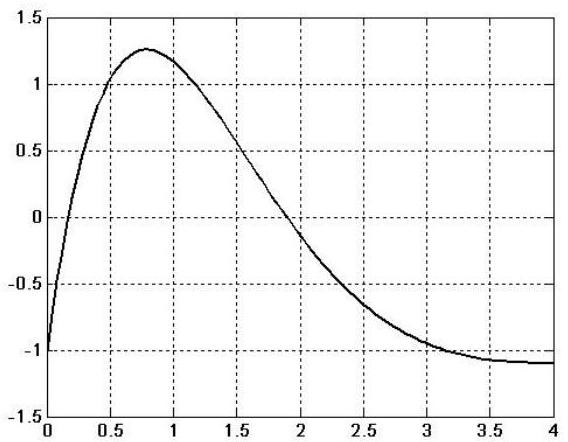
\includegraphics[width=0.5\linewidth]{fig_6_2}
		\label{fig:fig_6_2}
	\end{figure}
	\bigbreak
\bigbreak
The lowest positive root seems to be at approximately $0.2$.
\bigbreak
\item The formula for Newton-Raphson is
\bigbreak
$x_{i+1}=x_{i}-\dfrac{7 \sin \left(x_{i}\right) e^{-x_{i}}-1}{7 e^{-x_{i}}\left(\cos \left(x_{i}\right)-\sin \left(x_{i}\right)\right)}$
\bigbreak
Using an initial guess of $3.5$, the first iteration yields
\bigbreak$
\begin{aligned}
&x_{1}=0.3-\dfrac{7 \sin (0.3) e^{-0.3}-1}{7 e^{-0.3}(\cos (0.3)-\sin (0.3))}=0.3-\dfrac{0.532487}{3.421627}=0.144376 \\\\
&\left|\varepsilon_{a}\right|=\left|\dfrac{0.144376-0.3}{0.144376}\right| \times 100 \%=107.8 \%
\end{aligned}$
\bigbreak
Second iteration:
\bigbreak$
\begin{aligned}
&x_{2}=0.144376-\dfrac{7 \sin (0.144376) e^{-0.144376}-1}{7 e^{-0.144376}(\cos (0.144376)-\sin (0.144376))}=0.144376-\dfrac{-0.12827}{5.124168}=0.169409 \\\\
&\left|\varepsilon_{a}\right|=\left|\dfrac{0.169409-0.144376}{0.169409}\right| \times 100 \%=14.776 \%
\end{aligned}$
\bigbreak
Third iteration:
\bigbreak
$x_{1}=0.169409-\dfrac{7 \sin (0.169409) e^{-0.169409}-1}{7 e^{-0.169409}(\cos (0.169409)-\sin (0.169409))}=0.169409-\dfrac{-0.00372}{4.828278}=0.170179$
\bigbreak
$\left|\varepsilon_{a}\right|=\left|\dfrac{0.170179-0.169409}{0.170179}\right| \times 100 \%=0.453 \%$
\bigbreak

\item For the secant method, the first iteration:
\bigbreak

$\begin{array}{ll}x_{-1}=0.4 &\quad f\left(x_{-1}\right)=0.827244 \\x_{0}=0.3 &\quad f\left(x_{0}\right)=0.532487\end{array}$

\bigbreak
$
\begin{aligned}
&x_{1}=0.3-\dfrac{0.532487(0.4-0.3)}{0.827244-0.532487}=0.119347 \\\\
&\left|\varepsilon_{a}\right|=\left|\dfrac{0.119347-0.3}{0.119347}\right| \times 100 \%=151.4 \%
\end{aligned}$

\bigbreak
Second iteration:
\bigbreak
$\begin{array}{ll}
x_{0}=0.3 &\quad f\left(x_{0}\right)=0.532487 \\
x_{1}=0.119347 &\quad f\left(x_{1}\right)=-0.26032
\end{array}$
\bigbreak
$
\begin{aligned}
x_{2}=0.119347-\dfrac{-0.26032(0.3-0.119347)}{0.532487-(-0.26032)}=0.178664 \\\\
&\hspace*{-8.1cm}\left|\varepsilon_{a}\right|=\left|\dfrac{0.178664-0.119347}{0.178664}\right| \times 100 \%=33.2 \%
\end{aligned}$
\bigbreak
Third iteration:
\bigbreak

$\begin{array}{ll}x_{1}=0.119347 &\quad f\left(x_{1}\right)=-0.26032 \\x_{2}=0.178664 &\quad f\left(x_{2}\right)=0.04047\end{array}$
\bigbreak
$
\begin{aligned}
&x_{3}=0.178664-\dfrac{0.04047(0.119347-0.178664)}{-0.26032-0.04047}=0.170683 \\\\ & \left|\varepsilon_{a}\right|=\left|\dfrac{0.170683-0.178664}{0.170683}\right| \times 100 \%=4.68 \%
\end{aligned}$
\bigbreak

\item For the modified secant method, the first iteration:
\bigbreak

$\begin{array}{ll}x_{0}=0.3 &\quad f\left(x_{0}\right)=0.532487 \\x_{0}+\delta x_{0}=0.303 &\quad f\left(x_{0}+\delta x_{0}\right)=0.542708\end{array}$
\bigbreak$
\begin{aligned}
&x_{1}=0.3-\dfrac{0.01(0.3) 0.532487}{0.542708-0.532487}=0.143698 \\\\
&\left|\varepsilon_{a}\right|=\left|\dfrac{0.143698-0.3}{0.143698}\right| \times 100 \%=108.8 \%
\end{aligned}$
\bigbreak


Second iteration:
\bigbreak

$\begin{array}{ll}x_{1}=0.143698 &\quad f\left(x_{1}\right)=-0.13175 \\x_{1}+\delta x_{1}=0.145135 &\quad f\left(x_{1}+\delta x_{1}\right)=-0.12439\end{array}$
\bigbreak$
\begin{aligned}
&x_{2}=0.143698-\dfrac{0.02(0.143698)(-0.13175)}{-0.12439-(-0.13175)}=0.169412 \\\\
&\left|\varepsilon_{a}\right|=\left|\dfrac{0.169412-0.143698}{0.169412}\right| \times 100 \%=15.18 \%
\end{aligned}$
\bigbreak

Third iteration:
\bigbreak
$\begin{array}{ll}x_{2}=0.169412 &\quad f\left(x_{2}\right)=-0.00371 \\x_{2}+\delta x_{2}=0.171106 &\quad f\left(x_{2}+\delta x_{2}\right)=0.004456\end{array}$
\bigbreak$
\begin{aligned}
&x_{3}=0.169412-\dfrac{0.02(0.169412)(-0.00371)}{0.004456-(-0.00371)}=0.170181 \\\\
&\left|\varepsilon_{a}\right|=\left|\dfrac{0.170181-0.169412}{0.170181}\right| \times 100 \%=0.452 \%
\end{aligned}$
\bigbreak
\end{enumerate}


\section{}
\begin{enumerate}[label=\bfseries(\alph*)]
\item The formula for Newton-Raphson is
\bigbreak
$x_{i+1}=x_{i}-\dfrac{x_{i}^{5}-16.05 x_{i}^{4}+88.75 x_{i}^{3}-192.0375 x_{i}^{2}+116.35 x_{i}+31.6875}{5 x_{i}^{4}-64.2 x_{i}^{3}+266.25 x_{i}^{2}-384.075 x_{i}+116.35}$
\bigbreak
Using an initial guess of $0.5825$, the first iteration yields
\bigbreak$
\begin{aligned}
&x_{1}=0.5825-\dfrac{50.06217}{-29.1466}=2.300098 \\\\
&\left|\varepsilon_{a}\right|=\left|\dfrac{2.300098-0.5825}{2.300098}\right| \times 100 \%=74.675 \%
\end{aligned}$
\bigbreak
Second iteration
\bigbreak$
\begin{aligned}
&x_{1}=2.300098-\dfrac{-21.546}{0.245468}=90.07506 \\\\
&\left|\varepsilon_{a}\right|=\left|\dfrac{90.07506-2.300098}{90.07506}\right| \times 100 \%=97.446 \%
\end{aligned}$
\bigbreak
Thus, the result seems to be diverging. However, the computation eventually settles down and converges (at a very slow rate) on a root at $x=6.5$.\\ The iterations can be summarized as
\bigbreak
$
\begin{array}{crrrc}
\Xhline{1.5pt} \text { iteration } & \multicolumn{1}{c}{x_{i}} & \multicolumn{1}{c}{f\left(x_{i}\right)} & \multicolumn{1}{c}{f\left(x_{i}\right)} & \left|\varepsilon_{a}\right| \\
\hline 0 & 0.582500 & 50.06217 & -29.1466 & \\
1 & 2.300098 & -21.546 & 0.245468 & 74.675 \% \\
2 & 90.07506 & 4.94 \mathrm{E}+09 & 2.84 \mathrm{E}+08 & 97.446 \% \\
3 & 72.71520 & 1.62 \mathrm{E}+09 & 1.16 \mathrm{E}+08 & 23.874 \% \\
4 & 58.83059 & 5.3 \mathrm{E}+08 & 47720880 & 23.601 \% \\
5 & 47.72701 & 1.74 \mathrm{E}+08 & 19552115 & 23.265 \% \\
6 & 38.84927 & 56852563 & 8012160 & 22.852 \% \\
7 & 31.75349 & 18616305 & 3284098 & 22.346 \% \\
8 & 26.08487 & 6093455 & 1346654 & 21.731 \% \\
9 & 21.55998 & 1993247 & 552546.3 & 20.987 \% \\
10 & 17.95260 & 651370.2 & 226941 & 20.094 \% \\
11 & 15.08238 & 212524.6 & 93356.59 & 19.030 \% \\
12 & 12.80590 & 69164.94 & 38502.41 & 17.777 \% \\
13 & 11.00952 & 22415.54 & 15946.36 & 16.317 \% \\
14 & 9.603832 & 7213.396 & 6652.03 & 14.637 \% \\
15 & 8.519442 & 2292.246 & 2810.851 & 12.728 \% \\
16 & 7.703943 & 710.9841 & 1217.675 & 10.585 \% \\
17 & 7.120057 & 209.2913 & 556.1668 & 8.201 \% \\
18 & 6.743746 & 54.06896 & 286.406 & 5.580 \% \\
19 & 6.554962 & 9.644695 & 187.9363 & 2.880 \% \\
20 & 6.503643 & 0.597806 & 164.8912 & 0.789 \% \\
21 & 6.500017 & 0.00285 & 163.32 & 0.056 \% \\
22 & 6.5 & 6.58 \mathrm{E}-08 & 163.3125 & 0.000 \% \\
\Xhline{1.5pt}
\end{array}$
\bigbreak

\item For the modified secant method, the first iteration:
\bigbreak
$\begin{array}{ll}
x_{0}=0.5825 &\quad f\left(x_{0}\right)=50.06217 \\
x_{0}+\delta x_{0}=0.611625 & \quad f\left(x_{0}+\delta x_{0}\right)=49.15724 
\end{array}$
\bigbreak$
\begin{aligned}
& x_{1}=0.5825-\dfrac{0.05(0.5825) 50.06217}{49.15724-50.06217}=2.193735 \\\\
& \left|\varepsilon_{a}\right|=\left|\dfrac{2.193735-0.5825}{2.193735}\right| \times 100 \%=73.447 \% 
\end{aligned}$
\bigbreak
Second iteration:
\bigbreak
$\begin{array}{ll}
x_{1}=2.193735 & f\left(x_{1}\right)=-21.1969 \\
x_{1}+\delta x_{1}=2.303422 & f\left(x_{1}+\delta x_{1}\right)=-21.5448 
\end{array}$

\bigbreak$
\begin{aligned}
& x_{2}=2.193735-\dfrac{0.05(2.193735)(-21.1969)}{-21.5448-(-21.1969)}=-4.48891  \\\\ & \left|\varepsilon_{a}\right|=\left|\dfrac{-4.48891-2.193735}{-4.48891}\right| \times 100 \%=148.87 \%
\end{aligned}$

\bigbreak
Again, the result seems to be diverging. However, the computation eventually settles down and converges on a root at $x=-0.2$. The iterations can be summarized as
\bigbreak

\begin{tabular}{crrrrc}
\Xhline{1.5pt}
iteration & \multicolumn{1}{c}{$x_{i}$} & \multicolumn{1}{c}{$x_{i}+\delta x_{i}$} & $f\left(x_{i}\right)$ & $f\left(x_{i}+\delta x_{i}\right)$ & $\left|\varepsilon_{a}\right|$ \\
\hline
0 & $0.5825$ & $0.611625$ & $50.06217$ & $49.15724$ &  \\
1 & $2.193735$ & $2.303422$ & $-21.1969$ & $-21.5448$ & $73.447 \%$ \\
2 & $-4.48891$ & $-4.71336$ & $-20727.5$ & $-24323.6$ & $148.870 \%$ \\
3 & $-3.19524$ & $-3.355$ & $-7201.94$ & $-8330.4$ & $40.487 \%$ \\
4 & $-2.17563$ & $-2.28441$ & $-2452.72$ & $-2793.57$ & $46.865 \%$ \\
5 & $-1.39285$ & $-1.46249$ & $-808.398$ & $-906.957$ & $56.200 \%$ \\
6 & $-0.82163$ & $-0.86271$ & $-250.462$ & $-277.968$ & $69.524 \%$ \\
7 & $-0.44756$ & $-0.46994$ & $-67.4718$ & $-75.4163$ & $83.579 \%$ \\
8 & $-0.25751$ & $-0.27038$ & $-12.5942$ & $-15.6518$ & $73.806 \%$ \\
9 & $-0.20447$ & $-0.2147$ & $-0.91903$ & $-3.05726$ & $25.936 \%$ \\
10 & $-0.20008$ & $-0.21008$ & $-0.01613$ & $-2.08575$ & $2.196 \%$ \\
11 & $-0.2$ & $-0.21$ & $-0.0002$ & $-2.0686$ & $0.039 \%$ \\
12 & $-0.2$ & $-0.21$ & $-2.4 \mathrm{E}-06$ & $-2.06839$ & $0.000 \%$ \\
\Xhline{1.5pt}
\end{tabular}
\bigbreak
Explanation of results: The results are explained by looking at a plot of the function. The guess of $0.5825$ is located at a point where the function is relatively flat. Therefore, the first iteration results in a prediction of $2.3$ for Newton-Raphson and $2.193$ for the secant method. At these points the function is very flat and hence, the Newton-Raphson results in a very high value ( $90.075)$, whereas the modified false position goes in the opposite direction to a negative value $(-4.49)$. Thereafter, the methods slowly converge on the nearest roots.
\bigbreak
\begin{figure}[H]
		\hspace*{0.7cm}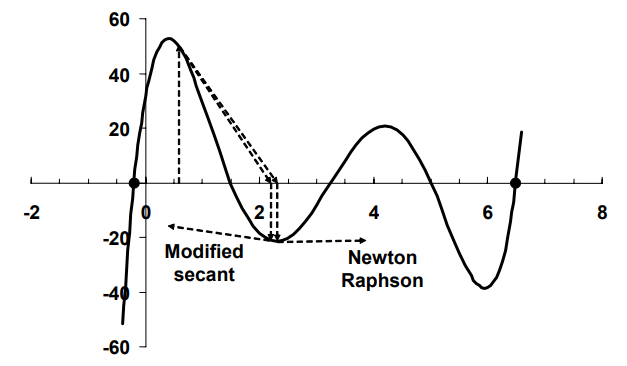
\includegraphics[width=0.6\linewidth]{fig_6_3}
		\label{fig:fig_6_3}
	\end{figure}
	\bigbreak


\section{}
\begin{lstlisting}[numbers=none]
function root = secant(func,xrold,xr,es,maxit)
% secant(func,xrold,xr,es,maxit):
%   uses secant method to find the root of a function
% input:
%   func = name of function
%   xrold, xr = initial guesses
%   es = (optional) stopping criterion (%)
%   maxit = (optional) maximum allowable iterations
% output:
%   root = real root

% if necessary, assign default values
if nargin<5, maxit=50; end 		 %if maxit blank set to 50
if nargin<4, es=0.001; end 		 %if es blank set to 0.001

% Secant method
iter = 0;
while (1)
  xrn = xr - func(xr)*(xrold - xr)/(func(xrold) - func(xr));
  iter = iter + 1;
  if xrn ~= 0, ea = abs((xrn - xr)/xrn) * 100; end
  if ea <= es | iter >= maxit, break, end
  xrold = xr;
  xr = xrn;
end
root = xrn;
\end{lstlisting}
\bigbreak
Test by solving Prob. 6.3:
\bigbreak
\begin{lstlisting}[numbers=none]
>> secant(inline('x^3-6*x^2+11*x-6.1'),2.5,3.5)

ans =
 	  3.0467
\end{lstlisting}
\bigbreak

\section{}
\begin{lstlisting}[numbers=none]
function root = modsec(func,xr,delta,es,maxit)
% secant(func,xrold,xr,es,maxit):
%   uses the modified secant method
%   to find the root of a function
% input:
%   func = name of function
%   xr = initial guess
%   delta = perturbation fraction
%   es = (optional) stopping criterion (%)
%   maxit = (optional) maximum allowable iterations
% output:
%   root = real root

% if necessary, assign default values
if nargin<5, maxit=50; end 		 %if maxit blank set to 50
if nargin<4, es=0.001; end 		 %if es blank set to 0.001
if nargin<3, delta=1E-5; end 	 %if delta blank set to 0.00001

% Secant method
iter = 0;
while (1)
  xrold = xr;
  xr = xr - delta*xr*func(xr)/(func(xr+delta*xr)-func(xr));
  iter = iter + 1;
  if xr ~= 0, ea = abs((xr - xrold)/xr) * 100; end
  if ea <= es | iter >= maxit, break, end
end
root = xr;
\end{lstlisting}
\bigbreak
Test by solving Prob. 6.3:
\bigbreak
\begin{lstlisting}[numbers=none]
>> modsec(inline('x^3-6*x^2+11*x-6.1'),3.5,0.02)

ans =
 	  3.0467

\end{lstlisting}
\bigbreak

\section{}
The equation to be differentiated is
\bigbreak
$f(m)=\sqrt{\dfrac{g m}{c_{d}}} \tanh \left(\sqrt{\dfrac{g c_{d}}{m} t}\right )-v$
\bigbreak
Note that
\bigbreak
$\dfrac{d \tanh u}{d x}=\operatorname{sech}^{2} u \dfrac{d u}{d x}$
\bigbreak
Therefore, the derivative can be evaluated as
\bigbreak
$\dfrac{d f(m)}{d m}=\sqrt{\dfrac{g m}{c_{d}}} \operatorname{sech}^{2}\left(\sqrt{\dfrac{g c_{d}}{m}} t\right)\left(-\dfrac{1}{2} \sqrt{\dfrac{m}{c_{d} g}}\right) t \dfrac{c_{d} g}{m^{2}}+\tanh \left(\sqrt{\dfrac{g c_{d}}{m} t}\right) \dfrac{1}{2} \sqrt{\dfrac{c_{d}}{g m}} \dfrac{g}{c_{d}}$
\bigbreak
The two terms can be reordered
\bigbreak
$\dfrac{d f(m)}{d m}=\dfrac{1}{2} \sqrt{\dfrac{c_{d}}{g m}} \dfrac{g}{c_{d}} \tanh \left(\sqrt{\dfrac{g c_{d}}{m}} t\right)-\dfrac{1}{2} \sqrt{\dfrac{g m}{c_{d}}} \sqrt{\dfrac{m}{c_{d} g}} \dfrac{c_{d} g}{m^{2}} t \operatorname{sech}^{2}\left(\sqrt{\dfrac{g c_{d}}{m}} t\right)$
\bigbreak
The terms premultiplying the tanh and sech can be simplified to yield the final result
\bigbreak
$\dfrac{d f(m)}{d m}=\dfrac{1}{2} \sqrt{\dfrac{g}{m c_{d}}} \tanh \left(\sqrt{\dfrac{g c_{d}}{m}} t\right)-\dfrac{g}{2 m} t \operatorname{sech}^{2}\left(\sqrt{\dfrac{g c_{d}}{m}} t\right)$
\bigbreak
\end{enumerate}

\section{}
\begin{enumerate}[label=\bfseries(\alph*)]
\item The formula for Newton-Raphson is
\bigbreak
$x_{i+1}=x_{i}-\dfrac{-2+6 x_{i}-4 x_{i}^{2}+0.5 x_{i}^{3}}{6-8 x_{i}+1.5 x_{i}^{2}}$
\bigbreak
Using an initial guess of $4.5$, the iterations proceed as
\bigbreak
\begin{tabular}{crrrc}
\Xhline{1.5pt}
iteration & \multicolumn{1}{c}{$x_{i}$} & \multicolumn{1}{c}{$f\left(x_{i}\right)$} & \multicolumn{1}{c}{$f\left(x_{i}\right)$} & $\left|\varepsilon_{a}\right|$ \\
\hline
0 & $4.5$ & $-10.4375$ & $0.375$ &  \\
1 & $32.333330$ & $12911.57$ & $1315.5$ & $86.082 \%$ \\
2 & $22.518380$ & $3814.08$ & $586.469$ & $43.586 \%$ \\
3 & $16.014910$ & $1121.912$ & $262.5968$ & $40.609 \%$ \\
4 & $11.742540$ & $326.4795$ & $118.8906$ & $36.384 \%$ \\
5 & $8.996489$ & $92.30526$ & $55.43331$ & $30.524 \%$ \\
6 & $7.331330$ & $24.01802$ & $27.97196$ & $22.713 \%$ \\
7 & $6.472684$ & $4.842169$ & $17.06199$ & $13.266 \%$ \\
8 & $6.188886$ & $0.448386$ & $13.94237$ & $4.586 \%$ \\
9 & $6.156726$ & $0.005448$ & $13.6041$ & $0.522 \%$ \\
10 & $6.156325$ & $8.39 \mathrm{E}-07$ & $13.59991$ & $0.007 \%$ \\
\Xhline{1.5pt}
\end{tabular}
\bigbreak
Thus, after an initial jump, the computation eventually settles down and converges on a root at $x=6.156325$.
\bigbreak
\item Using an initial guess of $4.43$, the iterations proceed as
\bigbreak

\begin{tabular}{crrrr}
\Xhline{1.5pt}
iteration & \multicolumn{1}{c}{$x_{i}$} & \multicolumn{1}{c}{$f\left(x_{i}\right)$} & \multicolumn{1}{c}{$f\left(x_{i}\right)$} & \multicolumn{1}{c}{$\left|\varepsilon_{a}\right|$} \\
\hline
0 & $4.43$ & $-10.4504$ & $-0.00265$ &  \\
1 & $-3939.13$ & $-3.1 E+10$ & 23306693 & $100.112 \%$ \\
2 & $-2625.2$ & $-9.1 E+09$ & 10358532 & $50.051 \%$ \\
3 & $-1749.25$ & $-2.7 E+09$ & 4603793 & $50.076 \%$ \\
4 & $-1165.28$ & $-8 E+08$ & 2046132 & $50.114 \%$ \\
5 & $-775.964$ & $-2.4 E+08$ & $909393.5$ & $50.171 \%$ \\
$.$ &  &  &  &  \\
$.$ &  &  &  &  \\
$.$ &  &  &  &  \\
21 & $0.325261$ & $-0.45441$ & $3.556607$ & $105.549 \%$ \\
22 & $0.453025$ & $-0.05629$ & $2.683645$ & $28.203 \%$ \\
23 & $0.474$ & $-0.00146$ & $2.545015$ & $4.425 \%$ \\
24 & $0.474572$ & $-1.1 \mathrm{E}-06$ & $2.541252$ & $0.121 \%$ \\
25 & $0.474572$ & $-5.9 \mathrm{E}-13$ & $2.541249$ & $0.000 \%$ \\
\Xhline{1.5pt}
\end{tabular}
\bigbreak
This time the solution jumps to an extremely large negative value The computation eventually converges at a very slow rate on a root at $x=0.474572$.
\bigbreak
Explanation of results: The results are explained by looking at a plot of the function. Both guesses are in a region where the function is relatively flat. Because the two guesses are on opposite sides of a minimum, both are sent to different regions that are far from the initial guesses. Thereafter, the methods slowly converge on the nearest roots.
\bigbreak
\begin{figure}[H]
		\hspace*{0.8cm}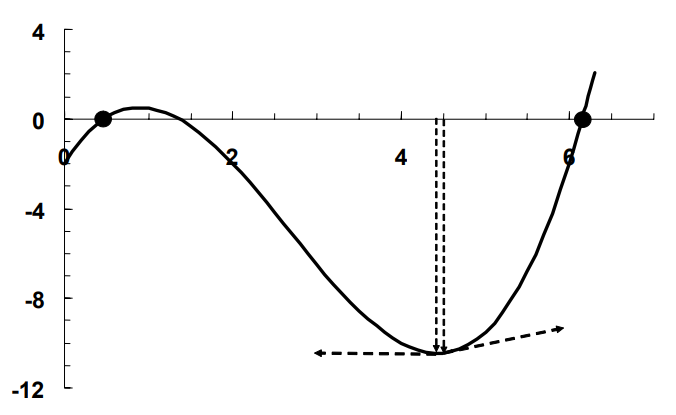
\includegraphics[width=0.6\linewidth]{fig_6_4}
		\label{fig:fig_6_4}
	\end{figure}
	\bigbreak

\bigbreak
\section{}
The function to be evaluated is
\bigbreak
$x=\sqrt{a}$
\bigbreak
This equation can be squared and expressed as a roots problem,
\bigbreak
$f(x)=x^{2}-a$
\bigbreak
The derivative of this function is
\bigbreak
$f^{\prime}(x)=2 x$
\bigbreak
These functions can be substituted into the Newton-Raphson equation (Eq. 6.6),
\bigbreak
$x_{i+1}=x_{i}-\dfrac{x_{i}^{2}-a}{2 x_{i}}$
\bigbreak
which can be expressed as
\bigbreak
$x_{i+1}=\dfrac{x_{i}+a / x_{i}}{2}$
\bigbreak
\end{enumerate}


\section{}
\begin{enumerate}[label=\bfseries(\alph*)]
\item The formula for Newton-Raphson is
\bigbreak
$x_{i+1}=x_{i}-\dfrac{\tanh \left(x_{i}^{2}-9\right)}{2 x_{i} \operatorname{sech}^{2}\left(x_{i}^{2}-9\right)}$
\bigbreak
Using an initial guess of $3.2$, the iterations proceed as
\bigbreak
\begin{tabular}{crrrc}
iteration & \multicolumn{1}{c}{$x_{i}$} & \multicolumn{1}{c}{$f\left(x_{i}\right)$} & $f^{\prime}\left(x_{i}\right)$ & $\left|\varepsilon_{a}\right|$ \\
0 & $3.2$ & $0.845456$ & $1.825311$ &  \\
1 & $2.736816$ & $-0.906910$ & $0.971640$ & $16.924 \%$ \\
2 & $3.670197$ & $0.999738$ & $0.003844$ & $25.431 \%$ \\ 
3 & $-256.413$ & & & $ 101.431 \%$
\end{tabular}
\bigbreak
\item The solution diverges from its real root of $x=3$. Due to the concavity of the slope, the next iteration will always diverge. The following graph illustrates how the divergence evolves.
\bigbreak
\begin{figure}[H]
		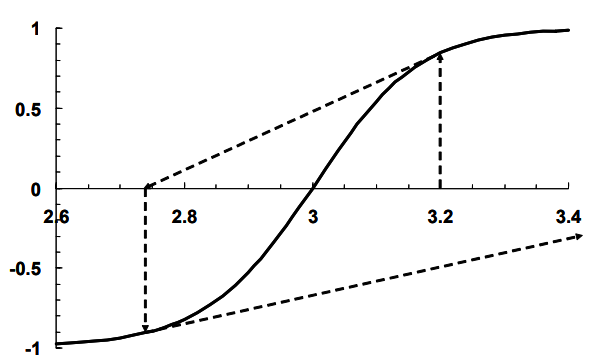
\includegraphics[width=0.5\linewidth]{fig_6_5 }
		\label{fig:fig_6_5}
	\end{figure}
	\bigbreak


\section{}
The formula for Newton-Raphson is
\bigbreak
$x_{i+1}=x_{i}-\dfrac{0.0074 x_{i}^{4}-0.284 x_{i}^{3}+3.355 x_{i}^{2}-12.183 x_{i}+5}{0.0296 x_{i}^{3}-0.852 x_{i}^{2}+6.71 x_{i}-12.1832}$
\bigbreak
Using an initial guess of $16.15$, the iterations proceed as
\bigbreak
\begin{tabular}{crcrr}
iteration & \multicolumn{1}{c}{$x_{i}$} & $f\left(x_{i}\right)$ & \multicolumn{1}{c}{$f\left(x_{i}\right)$} & \multicolumn{1}{c}{$\left|\varepsilon_{a}\right|$} \\
0 & $16.15$ & $-9.57445$ & $-1.35368$ &  \\
1 & $9.077102$ & $8.678763$ & $0.662596$ & $77.920 \%$ \\
2 & $-4.02101$ & $128.6318$ & $-54.864$ & $325.742 \%$ \\
3 & $-1.67645$ & $36.24995$ & $-25.966$ & $139.852 \%$ \\
4 & $-0.2804$ & $8.686147$ & $-14.1321$ & $497.887 \%$ \\
5 & $0.334244$ & $1.292213$ & $-10.0343$ & $183.890 \%$ \\
6 & $0.463023$ & $0.050416$ & $-9.25584$ & $27.813 \%$ \\
7 & $0.46847$ & $8.81 E-05$ & $-9.22351$ & $1.163 \%$ \\
8 & $0.46848$ & $2.7 E-10$ & $-9.22345$ & $0.002 \%$ \\
\end{tabular}
\bigbreak
As depicted below, the iterations involve regions of the curve that have flat slopes. Hence, the solution is cast far from the roots in the vicinity of the original guess.
\bigbreak
\begin{figure}[H]
		\hspace*{0.8cm}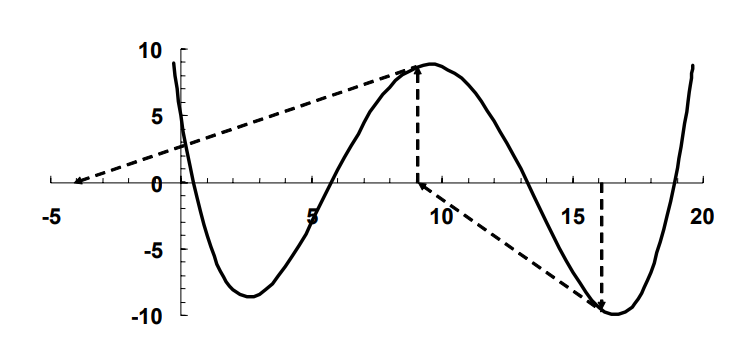
\includegraphics[width=0.7\linewidth]{fig_6_6}
		\label{fig:fig_6_6}
	\end{figure}
	\bigbreak


\section{}
The solution involves determining the root of
\bigbreak
$f(x)=\dfrac{x}{1-x} \sqrt{\dfrac{6}{2+x}}-0.05$
\bigbreak
MATLAB can be used to develop a plot that indicates that a root occurs in the vicinity of $x$ $=0.03$.

\begin{lstlisting}[numbers=none]
>> f = inline('x./(1-x).*sqrt(6./(2+x))-0.05')

f =
	  Inline function:
 	  f(x) = x./(1-x).*sqrt(6./(2+x))-0.05
 
>> x = linspace(0,.2);
>> y = f(x);
>> plot(x,y) 
\end{lstlisting}
\bigbreak
\begin{figure}[H]
		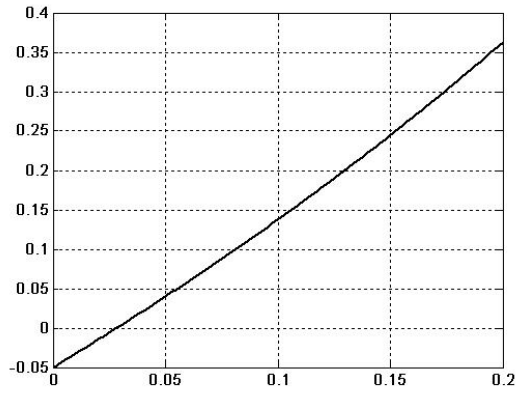
\includegraphics[width=0.5\linewidth]{fig_6_7}
		\label{fig:fig_6_7}
	\end{figure}
	\bigbreak

\bigbreak
The \textit{fzero} function can then be used to find the root
\bigbreak


\begin{lstlisting}[numbers=none]
>> format long
>> fzero(f,0.03)

ans =
	  0.02824944114847
\end{lstlisting}

\bigbreak
\section{}
The coefficient, $a$ and $b$, can be evaluated as
\begin{lstlisting}[numbers=none]
>> format long
>> R = 0.518;pc = 4600;Tc = 191;
>> a = 0.427*R^2*Tc^2.5/pc

a =
   12.55778319740302
 
>> b = 0.0866*R*Tc/pc

b =
   0.00186261539130
\end{lstlisting}
\bigbreak
The solution, therefore, involves determining the root of
\bigbreak
$f(v)=65,000-\dfrac{0.518(233.15)}{v-0.0018626}+\dfrac{12.557783}{v(v+0.0018626) \sqrt{233.15}}$
\bigbreak
MATLAB can be used to generate a plot of the function and to solve for the root. One way to do this is to develop an M-file for the function,
\bigbreak
\begin{lstlisting}[numbers=none]
function y = fvol(v)
R = 0.518;pc = 4600;Tc = 191;
a = 0.427*R^2*Tc^2.5/pc;
b = 0.0866*R*Tc/pc;
T = 273.15-40;p = 65000;
y = p - R*T./(v-b)+a./(v.*(v+b)*sqrt(T));
\end{lstlisting}
\bigbreak
This function is saved as fvol.m. It can then be used to generate a plot
\bigbreak
\begin{lstlisting}[numbers=none]
>> v = linspace(0.002,0.004);
>> fv = fvol(v);
>> plot(v,fv)
>> grid
\end{lstlisting}
\bigbreak
\begin{figure}[H]
		\hspace*{0.8cm}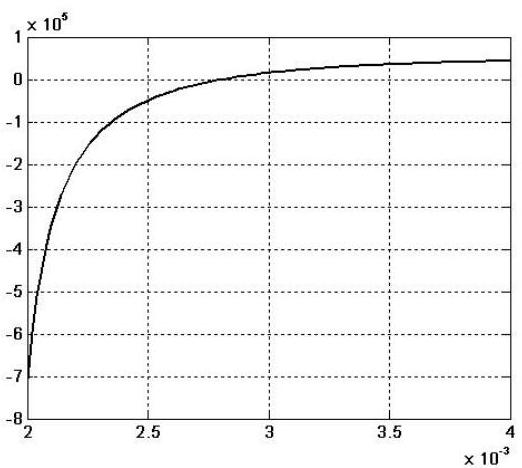
\includegraphics[width=0.5\linewidth]{fig_6_8}
		\label{fig:fig_6_8}
	\end{figure}
	\bigbreak

Thus, a root is located at about $0.0028$. The \textit {fzero} function can be used to refine this estimate,
\bigbreak
\begin{lstlisting}[numbers=none]
>> vroot = fzero('fvol',0.0028)

vroot =
    0.00280840865703
\end{lstlisting}
\bigbreak
The mass of methane contained in the tank can be computed as
\bigbreak
$\text { mass }=\dfrac{V}{v}=\dfrac{3}{0.0028084}=1068.317 \mathrm{~m}^{3}$
\bigbreak


\section{}
The function to be evaluated is
\bigbreak
$f(h)=V-\left[r^{2} \cos ^{-1}\left(\dfrac{r-h}{r}\right)-(r-h) \sqrt{2 r h-h^{2}}\right] L$
\bigbreak
To use MATLAB to obtain a solution, the function can be written as an M-file
\bigbreak
\begin{lstlisting}[numbers=none]
function y = fh(h,r,L,V)
y = V - (r^2*acos((r-h)/r)-(r-h)*sqrt(2*r*h-h^2))*L;
\end{lstlisting}
\bigbreak
The \textit {fzero} function can be used to determine the root as
\bigbreak
\begin{lstlisting}[numbers=none]
>> format long
>> r = 2;L = 5;V = 8;
>> h = fzero('fh',0.5,[],r,L,V)

h =
   0.74001521805594 
\end{lstlisting}
\bigbreak
\end{enumerate}


\section{}
\begin{enumerate}[label=\bfseries(\alph*)]
\item The function to be evaluated is
\bigbreak
$f\left(T_{A}\right)=10-\dfrac{T_{A}}{10} \cosh \left(\dfrac{500}{T_{A}}\right)+\dfrac{T_{A}}{10}$
\bigbreak
The solution can be obtained with the \textit {fzero} function as
\bigbreak
\begin{lstlisting}[numbers=none]
>> format long
>> TA = fzero(inline('10-x/10*cosh(500/x)+x/10'),1000)

TA =
 	  1.266324360399887e+003
\end{lstlisting}
\bigbreak
\item A plot of the cable can be generated as
\bigbreak
\begin{lstlisting}[numbers=none]
>> x = linspace(-50,100);
>> w = 10;y0 = 5;
>> y = TA/w*cosh(w*x/TA) + y0 - TA/w;
>> plot(x,y),grid 
\end{lstlisting}
\bigbreak
\begin{figure}[H]
		\hspace*{0.8cm}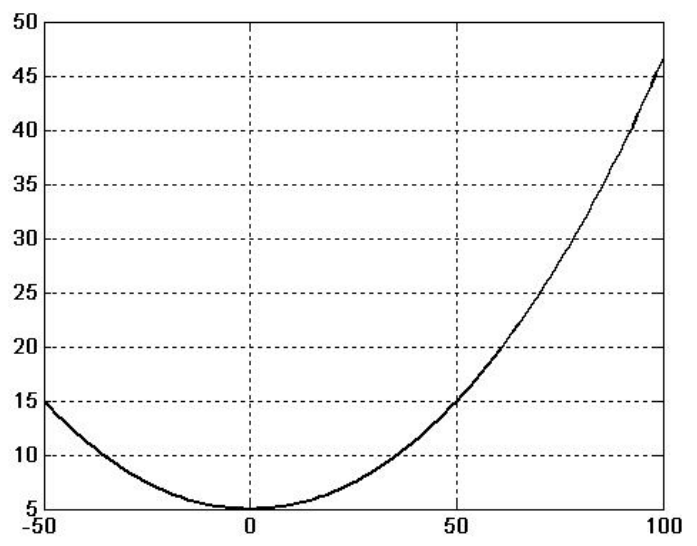
\includegraphics[width=0.5\linewidth]{fig_6_9}
		\label{fig:fig_6_9}
	\end{figure}
	\bigbreak


\section{}
The function to be evaluated is
\bigbreak
$f(t)=9 e^{-t} \sin (2 \pi t)-3.5$
\bigbreak
A plot can be generated with MATLAB,
\bigbreak
\begin{lstlisting}[numbers=none]
>> t = linspace(0,2);
>> y = 9*exp(-t) .* sin(2*pi*t) - 3.5;
>> plot(t,y),grid 
\end{lstlisting}
\bigbreak
\begin{figure}[H]
		\hspace*{0.8cm}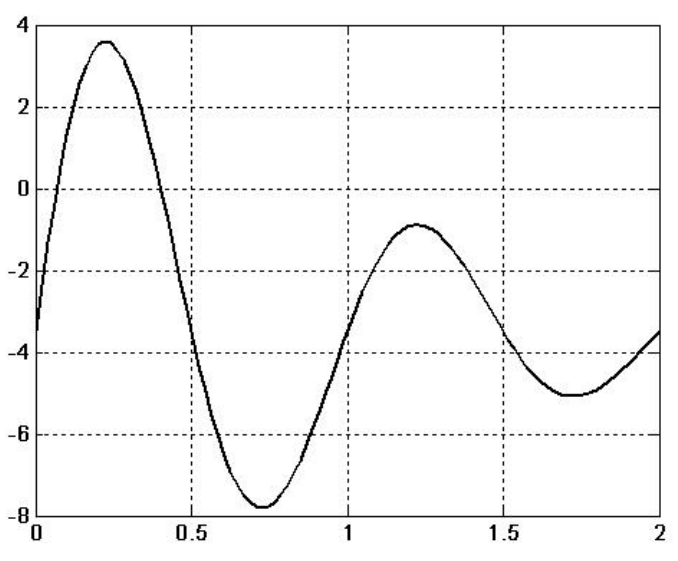
\includegraphics[width=0.5\linewidth]{fig_6_10}
		\label{fig:fig_6_10}
	\end{figure}
	\bigbreak
	
Thus, there appear to be two roots at approximately $0.1$ and $0.4$. The \textit {fzero} function can be used to obtain refined estimates,
\bigbreak
\begin{lstlisting}[numbers=none]
>> t = fzero('9*exp(-x)*sin(2*pi*x)-3.5',[0 0.2])

t =
 	 0.06835432096851
 	
>> t = fzero('9*exp(-x)*sin(2*pi*x)-3.5',[0.2 0.8])

t =
 	 0.40134369265980
\end{lstlisting}
\bigbreak

\section{}
The function to be evaluated is
\bigbreak
$f(\omega)=\dfrac{1}{Z}-\sqrt{\dfrac{1}{R^{2}}+\left(\omega C-\dfrac{1}{\omega L}\right)^{2}}$
\bigbreak
Substituting the parameter values yields
\bigbreak
$f(\omega)=0.01-\sqrt{\dfrac{1}{50625}+\left(0.6 \times 10^{-6} \omega-\dfrac{2}{\omega}\right)^{2}}$
\bigbreak
The \textit {fzero} function can be used to determine the root as
\bigbreak
\begin{lstlisting}[numbers=none]
>> fzero('0.01-sqrt(1/50625+(.6e-6*x-2./x).^2)',[1 1000])

ans =
  220.0202
\end{lstlisting}
\bigbreak


\section{}
The \textit {fzero} function can be used to determine the root as
\bigbreak
\begin{lstlisting}[numbers=none]
>> format long
>> fzero('2*40*x^(5/2)/5+0.5*40000*x^2-95*9.8*x-95*9.8*0.43',1)

ans =
   0.16662477900186
\end{lstlisting}
\bigbreak

\section{}
If the height at which the throw leaves the right fielders arm is defined as $y=0$, the $y$ at 90 $\mathrm{m}$ will be $-0.8$. Therefore, the function to be evaluated is
\bigbreak
$f(\theta)=0.8+90 \tan \left(\dfrac{\pi}{180} \theta_{0}\right)-\dfrac{44.1}{\cos ^{2}\left(\pi \theta_{0} / 180\right)}$
\bigbreak
Note that the angle is expressed in degrees. First, MATLAB can be used to plot this function versus various angles.
\bigbreak
\begin{figure}[H]
		\hspace*{0.8cm}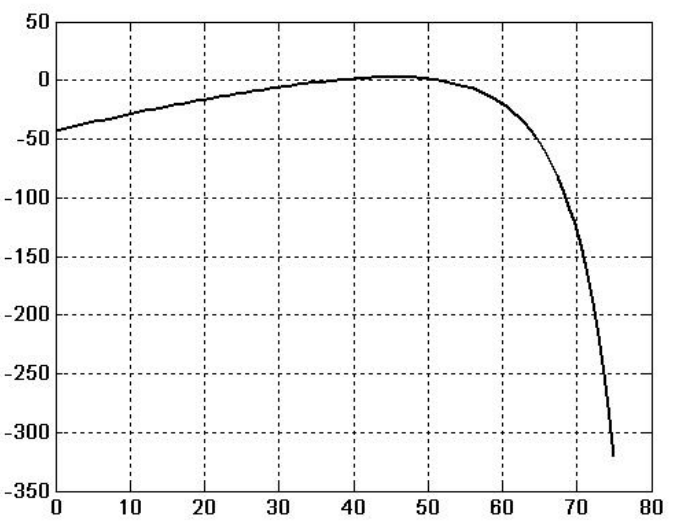
\includegraphics[width=0.5\linewidth]{fig_6_11}
		\label{fig:fig_6_11}
	\end{figure}
	\bigbreak
Roots seem to occur at about $40^{\circ}$ and $50^{\circ}$. These estimates can be refined with the fzero function,
\bigbreak
\begin{lstlisting}[numbers=none]
>> theta = fzero('0.8+90*tan(pi*x/180)-44.1./cos(pi*x/180).^2',0)

theta =
   37.8380
 
>> theta = fzero('0.8+90*tan(pi*x/180)-44.1./cos(pi*x/180).^2',[40 60])

theta =
   51.6527
\end{lstlisting}
Thus, the right fielder can throw at two different angles to attain the same result.
\bigbreak


\section{}
The equation to be solved is
\bigbreak
$f(h)=\pi R h^{2}-\left(\dfrac{\pi}{3}\right) h^{3}-V$
\bigbreak
Because this equation is easy to differentiate, the Newton-Raphson is the best choice to achieve results efficiently. It can be formulated as
\bigbreak
$x_{i+1}=x_{i}-\dfrac{\pi R x_{i}^{2}-\left(\dfrac{\pi}{3}\right) x_{i}^{3}-V}{2 \pi R x_{i}-\pi x_{i}^{2}}$
\bigbreak
or substituting the parameter values,
\bigbreak
$x_{i+1}=x_{i}-\dfrac{\pi(10) x_{i}^{2}-\left(\dfrac{\pi}{3}\right) x_{i}^{3}-1000}{2 \pi(10) x_{i}-\pi x_{i}^{2}}$
\bigbreak
The iterations can be summarized as
\bigbreak
\begin{tabular}{crrrc}
\Xhline{1.5pt}
iteration & \multicolumn{1}{c}{$x_{i}$} & \multicolumn{1}{c}{$f\left(x_{i}\right)$} & \multicolumn{1}{c}{$f\left(x_{i}\right)$} & \multicolumn{1}{c}{$\left|\varepsilon_{a}\right|$} \\
\hline
0 & 10 & $1094.395$ & $314.1593$ &  \\
1 & $6.516432$ & $44.26917$ & $276.0353$ & $53.458 \%$ \\
2 & $6.356057$ & $0.2858$ & $272.4442$ & $2.523 \%$ \\
3 & $6.355008$ & $1.26 \mathrm{E}-05$ & $272.4202$ & $0.017 \%$ \\
\Xhline{1.5pt}
\end{tabular}
\bigbreak
Thus, after only three iterations, the root is determined to be 6.355008 with an approximate
relative error of 0.017\%.
\bigbreak


\section{}
\begin{lstlisting}[numbers=none]
>> r = [-2 6 1 -4 8];
>> a = poly(r)

a =
    1 -9 -20 204 208 -384
    
>> polyval(a,1)

ans =
     0
 
>> b = poly([-2 6])

b =
    1 -4 -12
 
>> [q,r] = deconv(a,b)

q =
   1 -5 -28 32
r =
   0 0 0 0 0 0

>> x = roots(q)

x =
	  8.0000
 	 -4.0000
 	  1.0000
 	
>> a = conv(q,b)

a =
	  1 -9 -20 204 208 -384
	 
>> x = roots(a)

x =
 	  8.0000
	  6.0000
 	 -4.0000
 	 -2.0000
 	  1.0000
 	
>> a = poly(x)

a =
 	  1.0000 -9.0000 -20.0000 204.0000 208.0000 -384.0000

\end{lstlisting}
\bigbreak

\section{}
\begin{lstlisting}[numbers=none]
>> a = [1 9 26 24];
>> r = roots(a)

r =
 	 -4.0000
	 -3.0000
 	 -2.0000
 	
>> a = [1 15 77 153 90];
>> r = roots(a)

r =
 	 -6.0000
   -5.0000
   -3.0000
 	 -1.0000
\end{lstlisting}
\bigbreak
Therefore, the transfer function is
\bigbreak
$G(s)=\dfrac{(s+4)(s+3)(s+2)}{(s+6)(s+5)(s+3)(s+1)}$
\bigbreak

\end{enumerate}
\end{document}

